\section{2020 年 10 月 2 日答疑记录}

\subsection{二次函数的值域 (取值范围)}

求关于 $x$ 的二次函数 $f(x)= Ax^2+Bx+C$ ($A\neq 0$) 的值域时需利用定义域 ($x$ 的取值范围) 和单调性 (从左往右观察其图象时, 图象是上升还是下降), 而该函数的单调性可以通过观察其图象 (抛物线) 的开口方向和对称轴的位置得出, 其中由 $A$ 的正负号决定, 对称轴的公式为 $x= -\dfrac{B}{2A}$. 注意, 写对称轴时, 只需按照公式的格式写出对应的式子, 无需明确地写出公式. 如果对称轴容易口算, 也可直接写出, 如函数 $f(x)= x^2-2ax+1$ 的对称轴为 $x= a$.

具体地, 对二次函数 $y=f(x)= Ax^2+Bx+C$ ($A\neq 0$), 其中 $x\in[m,n]$, 参考下图 (为方便起见, 图中故意将不同定义域对应的函数图象画得与原图象分离)
 
  \begin{center}
  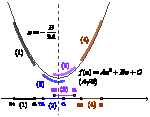
\includegraphics[scale=2.5]{2020-1018-0900-crop}
  \end{center}

(仅列出开口向上即 $A>0$ 的情形, 开口向下的情形结论类似)

(1) 若对称轴在定义域右侧, 即 $n\leqslant -\dfrac{B}{2A}$, 则
\[y_{\min}=f(n),\quad y_{\max}=f(m),\]
即 $y\in[f(n), f(m)]$;
  
(2) 若对称轴在定义域内部偏右, 即 $\dfrac{m+n}2\leqslant -\dfrac{B}{2A}< n$, 则
\[y_{\min}=f\biggl(-\dfrac{B}{2A}\biggr),\quad y_{\max}=f(m),\]
即 $y\in\biggl[f\biggl(-\dfrac{B}{2A}\biggr), f(m)\biggr]$;

(3) 若对称轴在定义域内部偏左, 即 $m\leqslant -\dfrac{B}{2A}< \dfrac{m+n}2$, 则
\[y_{\min}=f\biggl(-\dfrac{B}{2A}\biggr),\quad y_{\max}=f(n),\]
即 $y\in\biggl[f\biggl(-\dfrac{B}{2A}\biggr), f(n)\biggr]$;

(4) 若对称轴在定义域左侧, 即 $-\dfrac{B}{2A}<m$, 则
\[y_{\min}=f(m),\quad y_{\max}=f(n),\]
即 $y\in[f(m), f(n)]$.

讨论时应注意 ``不重不漏'' (不重复且不遗漏). 实际解题时, 不用写得很详细, 只写主要步骤即可, 见下一小节的例子.

\subsection{含参数的二次函数的值域}

一般遇到的二次函数值域问题, 有时函数表达式含参数 (代表已知数的字母, 但取值不固定), 有时定义域含参数, 偶尔两者兼有. 无论哪种情形, 都可以用上一小节的结论来解题, 即 ``看图说话''.

\begin{example}\label{exa:201018-1010}
  已知二次函数 $f(x)=x^2$, $x\in[-1,a)$, 求 $f(x)$ 的值域.
\end{example}
\begin{solution}
  由题意, $a>-1$, 故考虑 $a$ 从 $-1$ 开始不断增大时, 定义域与对称轴 $x=0$ 的位置关系.
  
  (1) 若 $-1<a\leqslant 0$, 则 $f(x)\in(f(a),f(-1)]= (a^2,1]$;
  
  (2) 若 $0<a\leqslant 1$, 则 $f(x)\in[f(0),f(-1)]= [0,1]$;
  
  (3) 若 $a> 1$, 则 $f(x)\in[f(0),f(a))= [0,a^2)$.
  
  综上所述,
  \[f(x)\in\begin{cases}
    (a^2,1], & a\in(-1,0],\\
    [0,1],   & a\in(0,1],\\
    [0,a^2), & a\in(1,+\infty).
    \end{cases}\]
\end{solution}
\begin{remark}
  (1) 例~\ref{exa:201018-1010} 只有上一小节的结论中 (1)---(3), 且容易看出对称轴在定义域正中间的时候, $a=1$, 所以按 $a\in(-1,0]$, $(0,1]$, $(1,+\infty]$ 三种情况讨论.
  
  (2) 最后的结论可以写为分段的形式, 方便查看, 其中大括号后先写值域, 再写参数范围; 也直接罗列 (见例~\ref{exa:201018-1100}).
\end{remark}

讨论时, 既可以将对称轴视为运动的, 也可以将定义域视为运动的. 一般建议将含参数的部分视为运动的. 在不熟悉解题过程之前, 解题时应画草图帮助思考.

\begin{example}\label{exa:201018-1100}
  已知二次函数 $f(x)=x^2-2x+2$, $x\in[t,t+1]$, 求 $f(x)$ 的值域.
\end{example}
\begin{solution}
  $f(x)$ 的对称轴为 $x=1$, 考虑其与定义域的位置可知
  
  (1) 若 $t+1\leqslant 1$ 即 $t\leqslant 0$, 则 
  \[f(x)\in[f(t+1),f(t)]= [t^2+1,t^2-2t+2];\]
  
  (2) 若 $\dfrac{t+(t+1)}2\leqslant 1< t+1$ 即 $0< t\leqslant \dfrac12$, 则 
  \[f(x)\in[f(1),f(t)]= [1,t^2-2t+2];\]
  
  (3) 若 $t\leqslant 1\leqslant \dfrac{t+(t+1)}2$ 即 $\dfrac12< t\leqslant 1$, 则 
  \[f(x)\in[f(1),f(t+1)]= [1,t^2+1];\]
  
  (4) 若 $t> 1$, 则 
  \[f(x)\in[f(t),f(t+1)]= [t^2-2t+2,t^2+1].\]
  
  综上所述, 若 $t\in(-\infty,0]$, 则 $f(x)\in[t^2+1,t^2-2t+2]$; 
  
  若 $t\in\biggr(0,\dfrac12\biggr]$, 则 $f(x)\in[1,t^2-2t+2]$;
  
  若 $t\in\biggr(\dfrac12,1\biggr]$, 则 $f(x)\in[1,t^2+1]$; 
  
  若 $t\in (1,+\infty)$, 则 $f(x)\in[t^2-2t+2,t^2+1]$.
\end{solution}

熟悉以上解题步骤后, 可以直接脑补草图, 并根据对称轴与定义域 (及其中点) 的位置关系写解题过程.

\begin{example}
  已知二次函数 $f(x)=x^2-2ax-1$ ($a\in\realnum$), $x\in[0,2]$, 求 $f(x)$ 的值域.
\end{example}
\begin{solution}
  $f(x)$ 的对称轴为 $x=a$, 故
  
  (1) 若 $a\leqslant 0$, 则 
  \[f(x)\in[f(0),f(2)]= [-1,3-4a];\]
  
  (2) 若 $0<a\leqslant 1$, 则 
  \[f(x)\in[f(a),f(2)]= [-a^2-1,3-4a];\]
  
  (3) 若 $1<a \leqslant 2$, 则 
  \[f(x)\in[f(a),f(0)]= [-a^2-1,-1];\]
  
  (4) 若 $a> 2$, 则 
  \[f(x)\in[f(2),f(0)]= [3-4a,-1].\]
  
  综上所述, 
  \[f(x)\in\begin{cases}
    [-1,3-4a],     & a\in(-\infty,0],\\
    [-a^2-1,3-4a], & a\in (0,1],\\
    [-a^2-1,-1],   & a\in (1,2],\\
    [3-4a,-1],     & a\in (2,+\infty).
  \end{cases}\]
\end{solution}

\endinput